This chapter will introduce algorithms we used in our work, including the design of heterogeneous NoC, the main process of exploring the mapping-routing combined search space by Tabu search, and computing the best route of each map result by reinforcement learning.

\section{Heterogeneous NoC design}
Most of the existing researches about task mapping and routing are based on homogeneous NoC.
%这里可以列一些参考文献
In reality, heterogeneous NoCs are increasingly appearing in people’s life, especially on smart phones. Figure 4.1 is a heterogeneous example, which is big.LITTLE architecture proposed by ARM and is widely used in various devices. Threads with high priority or requiring high computing speed can be assigned to high-performance CPU cores, while threads with low priority or low computing speed requirements (such as background tasks) are completed by low-power CPU cores.

\begin{figure}
    \centering
    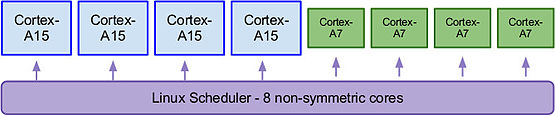
\includegraphics[]{../Figures/big_little.jpg}
    \caption{big.LITTLE architecture}
\end{figure}


In this paper, We used the method proposed by Shoukat Ali to practice our heterogeneous NoC design[]. Specifically, we use a coefficient-of-variation-based(CVB) generation method to get a matrix of expected time to compute(ETC). In ETC matrix, the element ETC[i][j] is the expected execution time of task i on PE j. PE's number calculation method is defined as the following formula:
\begin{center}
    $PE's\ Number=(row-1) \times mesh\ size + (column-1)$
\end{center}
For example, the number of PE in the second row and third column in 8x8 mesh network is (2-1)x8+(3-1)=10. 


The CVB generation method is described as the following pseudo code:
\begin{algorithm}
    \caption{CVB generation method}
    \LinesNumbered
    \KwIn{
        $q$, the vector of average execution time of all tasks \\
        $t$, number of tasks \\
        $V_{machine}$, NoC heterogeneity coefficient \\
        $m$, number of PEs \\
    }
    \KwOut{
        $ETC$, the matrix of expected time to compute
    }
    $\alpha_{machine}=\frac{1}{V_{machine}^2}$ \\
    \For{$i \in [0,t-1]$}{
        $\beta_{machine}[i]=\frac{q[i]}{\alpha_{machine}}$ \\
        \For{$j \in [0,m-1]$}{
            $ETC[i,j]=Gamma(\alpha_{machine},\beta_{machine}[i])$ \\
            /*$Gamma$(·) is Gamma distribution, independent sampling each time*/
        }
    }
\end{algorithm}


\section{Tabu search}
\subsection{Original Tabu search}
\subsection{Robust Tabu search}
As a variant of the original Tabu Search, The Robust Tabu search was proposed in [1] to
%E. Taillard, “Robust taboo search for the quadratic assignment problem”, Parallel Comput., vol. 17, no 4–5, p. 443–455, 1991
%还可以吹一下robust tabu search跟original tabu search有什么区别,这个在Exploring Tabu search Based...那篇文章好像有提?
explore search space in a more efficient method. In chapter X, we mentioned that the mapping problem, which is the problem of the mapping relationship between the Processing Element(PE) and the calculation task, is a quadratic assignment problem(QAP). Some existing studies, by comparing kinds of algorithms, have shown that the most efficient methods to solve a QAP are Tabu Search and its variants, which take both computational time and the quality of solution into consideration[2][3][4].
%[2]Fujiwara, I.; Koibuchi, M; “Mapping Non-trivial Network Topologies Onto Chips.” IEEE Int. Symp. on Embedded Multicore Socs (MCSoC 2013), pp.26-28
%[3]Modiri, A., Ansari-Asl, K, Nejad, E. B; “Improvement in 2D Network on Chip Using Tabu Search Mapping Algorithm” Int. J. of Computer Science and Network Solutions (IJCSNS), 2, (3), 2014 , pp. 75-87
%[4]Said, G. A. E. A et al; “A Comparative Study of Meta-heuristic Algorithms for Solving Quadratic Assignment Problem” Neural and Evolutionary Computing, 5 (1) 2014, pp. 1-6
Based on these studies, we were inspired to explore the effect of Tabu Search in the joint search space of mapping and routing.

\begin{figure}
    \centering
    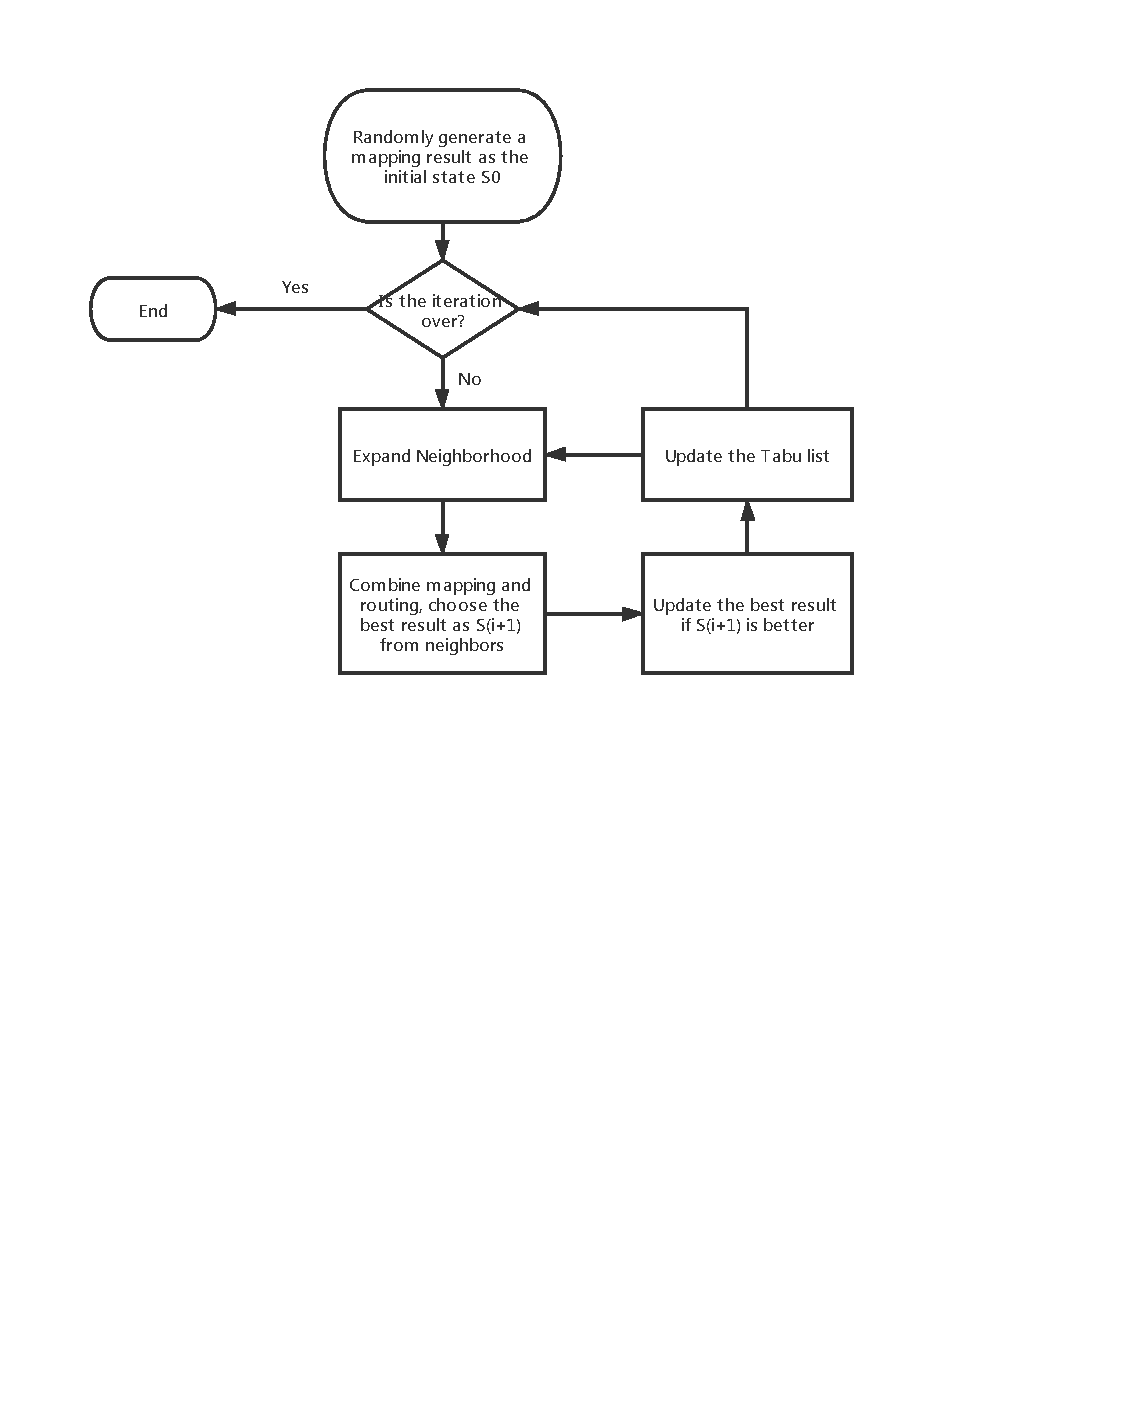
\includegraphics{../Figures/main_flowchart.pdf}%流程图里的符号应该改成跟表格里的一样
    \caption{The main process of Tabu search}
\end{figure}

\begin{figure}
    \centering
    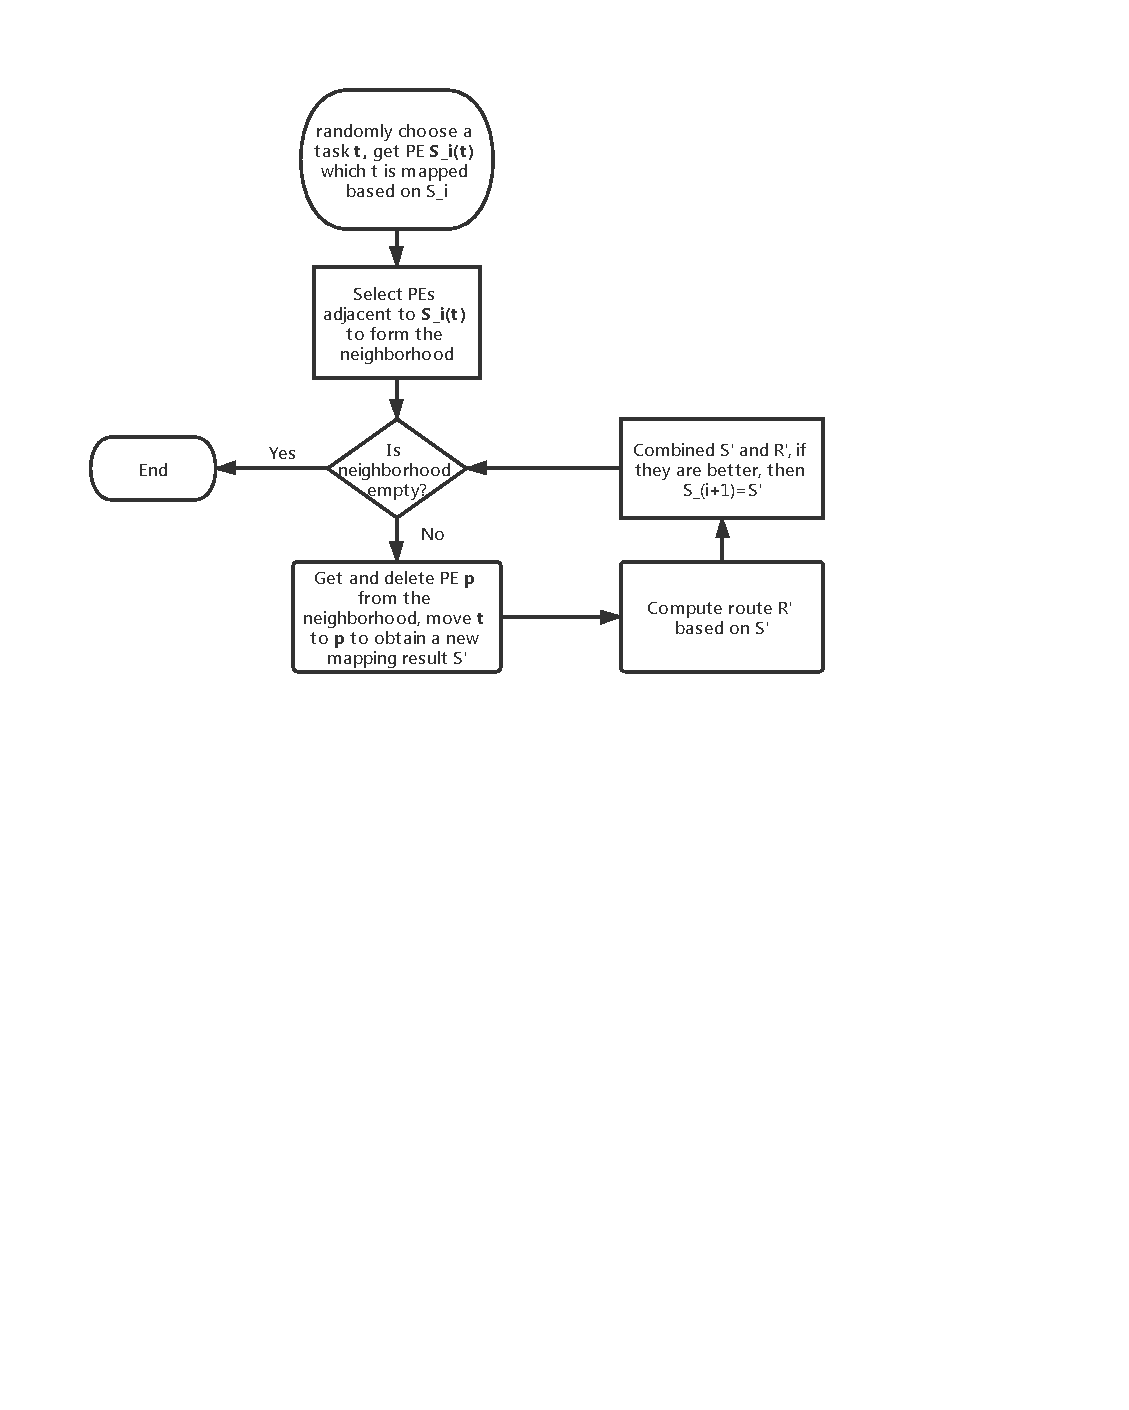
\includegraphics{../Figures/Expand_Neighborhood.pdf}
    \caption{Expand Neighborhood}
\end{figure}

Figure 4.2 shows how Robust Tabu search works to get the result. In order to show our algorithm in a more specific way, we provide both a flowchart and pseudo code to make it more convenient for readers. In order to avoid being overly complicated and easy to read, we split the flowchart into two parts. In flowcharts, you could simply replace Figure 4.3 with "Expand Neighborhood" in Figure 4.2. The pseudo code is at the end of this section.

The rounded rectangles represent the beginning state and the end state. The end state has been marked by the "end" word, so the other one is the beginning state. We randomly select a PE for each task, and then map the task to the PE. It is possible for multiple tasks to be mapped to the same PE, of course, this behavior is not advocated, due to its negative impact on program parallelism. After this work is completed, We use this randomly generated mapping result $\mathcal{M}_0$ as the initial state. 

After the initial operation, it comes to the iterative process. In Tabu search, the neighborhood of a certain state $\mathcal{M}$ is defined as a set which is  all possible states that can be obtained after one operation of the state $\mathcal{M}$. Based on this definition, the operation in our algorithm is, first randomly select a task $t$, then move this task to the PE adjacent to $\mathcal{M}(t)$.
%这里可以考虑画个图来解释operation
In 2D-mesh NoC, each PE has up to eight adjacent PEs. In extreme cases, it will be reduced to three. Therefore, based on this setting, each neighborhood has three to eight possible states to explore.


After the process of expand neighborhood, the algorithm should choose the best state from neighborhood. As a co-optimization algorithm, our algorithm will integrate mapping and routing to select the best state. Specifically, we will compute a best route for each mapping result by our routing algorithm mentioned in section 4.3, then consider these two aspects together.

%需要在符号表上加上p,用来衡量一个状态有多好
To define how good a result is ,we define a parameter $p$ which consists of two parts. The first part $p_1$ corresponds to mapping, it is the sum of the execution time of all tasks on the PE mapped to. The second part $p_2$ corresponds to routing, it is the sum of the waiting time caused by contention when transmitting data after a task is finished.

As we mentioned in section 4.1, the NoC we are experimenting with is heterogeneous, so the same task is mapped on different PEs, or the same PE is processing different tasks, and the execution time is both different. Our algorithm is expected to find the result that minimizes the execution time of all tasks, so $p_1$, the the sum of the execution time of all tasks, should be as small as possible. In order to avoid all tasks being concentrated to compete for certain PEs with strong computing ability, we punished this situation that multiple tasks are mapped on the same PE. In detail, when calculating $p_1$, The execution time of task $t$ will be multiplied by a coefficient, which is the number of tasks mapped on PE $\mathcal{M}(t)$. In this case, only multiple tasks are mapped on the same PE will be punished.

Our algorithm is a contention-aware algorithm, so $p_2$ is waiting time caused by contention. Different from the simulator which calculates cycle by cycle, we adopted another faster method to estimate waiting time. Detailed instructions will be mentioned in section 4.3.

According to the above description, the parameter $p$ is given by the following formula:
%应该在符号表里加上ET矩阵是什么
\begin{center}
    $p=\sum_{t}^{\mathcal{V}}ET[t][\mathcal{M}(t)]*task\_num(\mathcal{M}(t))+contention\_time$
\end{center}


The smaller the parameter $p$, the better the quality of this result. At the mapping level, this means finding a PE with strong computing ability; at the routing level, this means that there is less contention in the result we find.

When we find the best result among the neighborhood in the current state, we set it to the state of the next iteration, and then add this operation to the tabu list. The operation in tabu list will never be adopted until it is released from tabu list. This effectively ensure that our algorithm does not fall into local optima. To explain this more clearly, we use Figure 4.4 to give an example.

\begin{figure}
    \centering
    \subfigure[state 1]{
        \begin{minipage}[t]{0.48\linewidth}
            \centering
            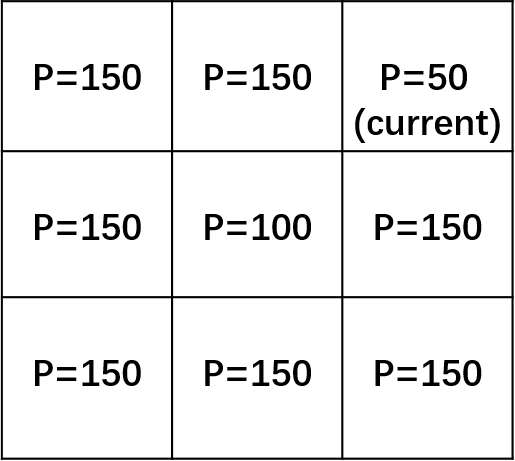
\includegraphics[width=6cm]{../Figures/example_for_tabulist1.png}
        \end{minipage}
    }
    \subfigure[state 2]{
        \begin{minipage}[t]{0.48\linewidth}
            \centering
            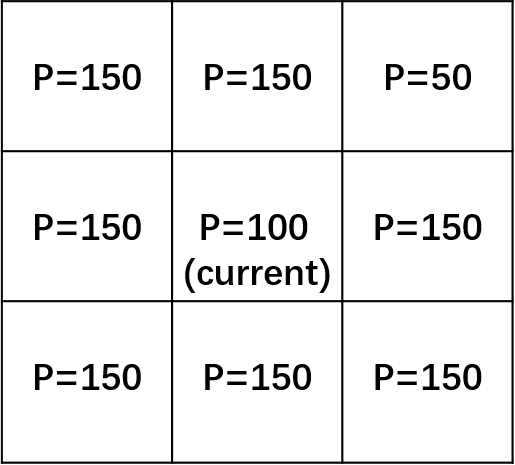
\includegraphics[width=6cm]{../Figures/example_for_tabulist2.png}
        \end{minipage}
    }
    \caption{Example for explaining tabu list}
\end{figure}

In Figure 4.4(a), the current state falls in the first row and third column. It's neighborhood has three elements, the best one is located in the second row and second column, the state in the next iteration has moved to this position. After this move operation, the current state falls in the second row and the second column, as shown in Figure 4.4(b). If we do not add this operation to the tabu list, the algorithm will still return to the first row and third column in the next iteration, because this is the best one in current neighborhood. The algorithm will move back and forth between these two positions, thus falling into an endless loop. The significance of the tabu list is to force the algorithm to accept a certain state that is not particularly good, so as to move to a new position to explore other search spaces in order to find the best state.

Finally, we record the best state $\mathcal{M}_b$ that has occurred during the iteration as the final mapping result. Then we use the routing algorithm mentioned in section 4.3 to obtain the corresponding route $\mathcal{R}(\mathcal{M}_b)$, so as to get the solution to this task graph.

\begin{algorithm}
    \caption{Robust Tabu Search}
    \LinesNumbered
    \KwIn{
        $\mathcal{V}, \mathcal{E}$,  The set of tasks nodes and edges. \newline
        $\mathcal{A}$, The set of processing elements.
    }
    \KwOut{Best mapping result $\mathcal{M}_b$ and its corresponding routing result $\mathcal{R}_b$}
    %这里应该在符号表里介绍一下M(·)是某个task映射到的PE
    \textbf{Initialize} {Randomly generate a $\mathcal{M}_0$ as the initially state \newline
    Tabu list($TL$)=$\emptyset$} \\
  \For{$i \in [0,max\_iteration]$}{
        $t=Random(\mathcal{V})$ //randomly choose a task from $\mathcal{V}$\\
        $\mathcal{M}^{'}=\emptyset,j^{'}=0$ \\
        \For{$j \in Neig( \mathcal{M}_{i}(t) ) \ AND\  (\mathcal{M}_i(t),j) \notin TL$}{
            $\mathcal{M}_i(t)=j$ \\
            $\mathcal{R}_i=\mathcal{G}(\mathcal{M}_i)$ \\
            %reward=$Reward\_func(\mathcal{M}_i,\mathcal{R}_i)$\\
            \If{$\mathcal{M}_i \ and\  \mathcal{R}_i$ is better}{
                $\mathcal{M}^{'}=\mathcal{M}_i,j^{'}=j$
            }
            restore $\mathcal{M}_i$
        }
        $\mathcal{M}_{i+1}=\mathcal{M}^{'}$ \\
        \If{$TL$ is full}{
            delete $TL[0]$
        }
        add $(\mathcal{M}_i(t),j^{'})$ to $TL$'s tail \\
        \If{$\mathcal{M}_{i+1}$ is better than $\mathcal{M}_{b}$}{
            $\mathcal{M}_{b}=\mathcal{M}_{i+1}$ \\
            $\mathcal{R}_b=\mathcal{G}(\mathcal{M}_b)$
        }
    }
\end{algorithm}

\section{Routing algorithm}
Our routing algorithm is based on Advantage Actor Critic(A2C) which is a reinforcement learning algorithm. This section will introduce reinforcement learning, A2C and how do we apply them to routing algorithm.

\subsection{Reinforcement learning}
Reinforcement learning is a algorithm aims to maximize the cumulative reward, it is studied in many disciplines, such as game theory, multi-agent systems and control theory. The basic reinforcement learning model should include:
\begin{itemize}
    \item The set of environment and agent states $S$, beginning with initial state $s_0$;
    \item A action function $A(s_t)$ gives all possible actions when agent is in state $s_t$;
    \item A reward function $R(s_t)$ gives reward of current state $s_t$;
    \item A transition model $P(s_{t+1}|s_t,a_t)$ gives the probability of state $s_t$ to state $s_{t+1}$ through action $a_t$
\end{itemize}
In this section, all $s$ and its variants with superscript or subscript represent state, all $a$ and its variants with superscript or subscript represent action. 

\begin{figure}[h]
    \centering
    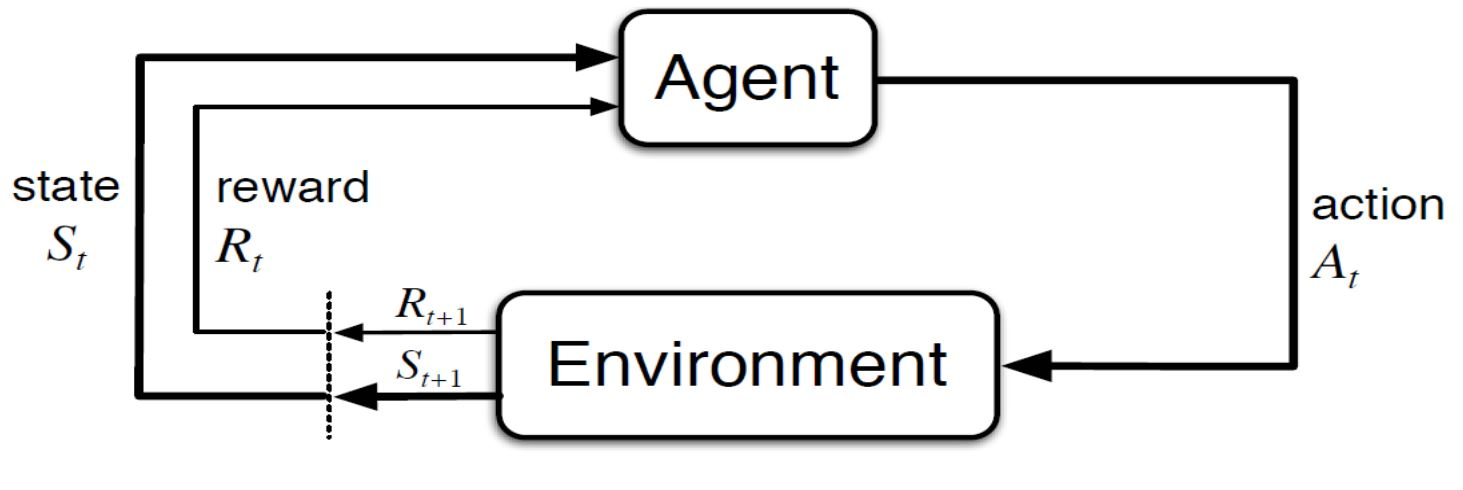
\includegraphics[width=\linewidth]{../Figures/agent_env.JPG}
    \caption{How agent and environment interact}
\end{figure}

The way agent and environment interact is shown in the Figure 4.. At time step $t$, agent observes state $s_t$ and produce action $a_t$, then it gets resulting reward $r_{t+1}$ and next state $s_{t+1}$. Figure 4. gives a timeline summary of 
multiple time steps. The probability of reach $s_{t+1}$ from $s_t$ depends only on current state $s_t$ and action $a_t$, not any other past states or actions.

\begin{figure}[h]
    \centering
    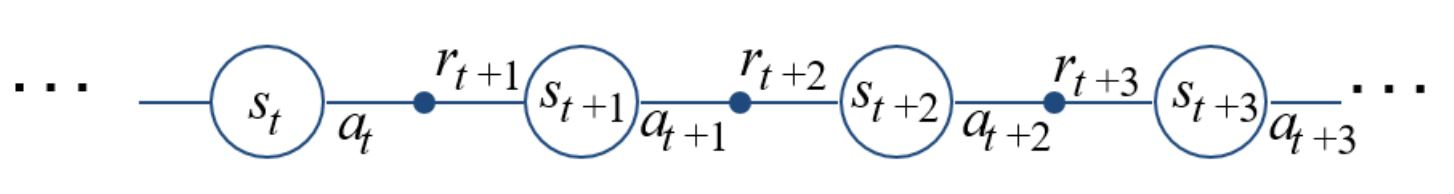
\includegraphics[width=\linewidth]{../Figures/timeline_RL.JPG}
    \caption{Timeline of multiple time steps}
\end{figure}

The algorithm design ideas of reinforcement learning are very similar to human thinking. In the beginning, the computer know nothing about everything, and learn from mistakes after constant trial and error, and finally found the pattern, thus having the ability to solve this type of problem. 

When the computer makes an action $a$ from state $s$ to state $s^{'}$, the reward function will give a definite reward to tell the computer whether it is good or bad to perform action $a$ in state $s$. The computer will remember this evaluation and update its own strategy. When in the state $s$ again, the computer will make better decisions based on past experience. Different from the supervised learning with labels on training samples, the data has no labels during the training process of reinforcement learning, and only learns through rewards and punishments given by the environment.

There are two basic methods in reinforcement learning, which are \textbf{value-based} and \textbf{policy-based}. Value-based algorithm record the corresponding reward after each action. When the agent need to perform action, value-based algorithm will directly select the most valuable action based on previous experience. It is usually used to deal with the situation where the action space is discrete, and when the action space is continuous, it can do nothing, because it can no longer record the corresponding value for every action.

In the case that the action space is continuous, we usually use the policy-based algorithm to solve the problem. Policy-based algorithm will analyze the current state, and then give the probability of various actions to be taken in the next step, after that take actions based on this probability distribution. In the training process, the policy-based algorithm will modify its parameters according to the reward of each action executed, and then it will give better results when the probability distribution of all actions needs to be given again.

Regardless of value-based or policy-based, our goal is finding a policy function $\pi (s)$ to give the excellent action that an agent takes in any given state $s$. However, when measuring the quality of a state $s$, we cannot only focus on the reward of this state $s$, but also the rewards of other states that can be reached through this state, which is the "potential" of this state $s$. We discount the individual state rewards by a factor $\gamma$ which is between 0 and 1, so we have the expected sum of discounted rewards $G(s_t)$. $G(s_t)$ is based on the assumption that the agent will execute the optimal policy from state $s_t$. It is shown by the following formula:
$$
G(s_t)
= R(s_t)+\gamma R(s_{t+1})+\gamma ^2R(s_{t+2})+...  
= \sum_{i=t}^\infty \gamma^{i-t}R(s_i) 
$$
If our current state is $s$, the state that may be reached after $s$ is $s'$, then the optimal policy will be :
$$
\pi^*(s)=\mathop{argmax}\limits_{a\in A(s)} \sum_{s'}P(s'|s,a)G(s')
$$


\subsubsection{Value-based algorithm}

For value-based algorithm, our goal is learning a policy $\pi(a|s)$ via a value function $Q(s,a)$. The value function $Q(s,a)$ is used to measure the value of performing action $a$ in state $s$. Take Q-learning as an example, this algorithm will maintain a Q table to get the best action $argmax_{a^*}Q(s,a)$. A simple Q table is shown as Table 4.1.
\begin{table}[h]
    \centering
    \caption{A simple Q table}\label{tab:aStrangeTable}
    \begin{tabular}{|c|c|c|}
        \hline
        Q-table & $a_1$ & $a_2$ \\
        \hline
        $s_1$ & 1 & 5 \\
        \hline
        $s_2$ & 2 & 3 \\
        \hline
        $s_3$ & 4 & 6 \\
        \hline
    \end{tabular}
\end{table}

When the agent is in state $s_1$, $\pi(a|s)$ will choose the action with a large Q value to execute, that is, $a_2$. When the agent transitions to a new state, it will still choose the action it will perform according to the Q table until the end. The classic methods of updating the value of the status include Monte Carlo Method and Temporal Difference Learning.

In Monte Carlo method, The update formula for the value is as follows:
$$
V(s_t) \leftarrow V(s_t)+\alpha \left[ G_t-V(s_t) \right]
$$
where $G_t=\sum_{k=0}^\infty \gamma^k R_{t+k+1}$ is the actual reward from time step $t$ and $\alpha$ is the given learning rate.

the reward will be calculated after the episode ends and then the model will be updated. This method has a disadvantage. When the model gets a high reward, the model will think all actions it takes are excellent, even if there are some actions is not good. Figure 4. gives a example to explain this phenomenon. Although $A_3$ is a bad action, the total reward is still high due to the excellent performance of other actions. In this situation, the model will consider $A_3$ as a good action. 

\begin{figure}
    \centering
    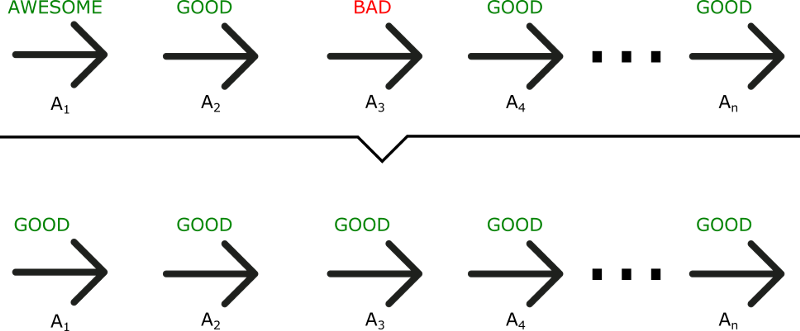
\includegraphics[width=\linewidth]{../Figures/bad_example_MC.png}
    \caption{An example for the disadvantage in Monte Carlo}
\end{figure}

In this situation, we need a large number of samples and enough learning time to make the model converge, which is undoubtedly disadvantageous. We hope to be able to update at each time step, so Temporal Difference Learning was proposed.

Temporal Difference Learning(TD Learning) is usually used to calculate the value of the state. When the time step transits from $t$ to $t+1$, TD learning could immediately update $V(s_t)$ based on the observed reward $R_{t+1}$ and estimated value $V(s_{t+1})$ as follows:
$$
V(s_t) \leftarrow V(s_t)+\alpha \left[ R_{t+1}+\gamma V(s_{t+1})-V(s_t) \right]
$$
where $\alpha$ is given learning rate and $\gamma$ is attenuation coefficient.

Based on these considerations, we use TD Learning to update Q table. Given learning rate $\alpha$, for state $s$, action $a$ and the next state $s'$ of $s$ through action $a$, we firstly get the reward $r$ from state $s$ performing action $a$, then update $Q(s,a)$ by following formula based on TD Learning:
$$
Q(s,a)\leftarrow Q(s,a)+\alpha \cdot [r+\gamma \cdot max_{a'}Q(s',a')-Q(s,a)]
$$
Based on this process, the pseudo code is shown in Algorithm 3.


\begin{algorithm}
    \caption{value-based algorithm}
    \LinesNumbered
    \KwIn{
        $S$, the set of environment and agent states \newline
        $A(\cdot)$, the action function \newline
        $R(\cdot)$, the reward function \newline
        $P(s'|s,a)$, the transition model
    }
    \KwOut{
        $Q(s,a)$, Q table
    }
    \textbf{Initialize}{
        $Q(s,a)$ arbitrarily
    } \\
    \For{$i \in [0,max\_episodes]$}{
        \textbf{Initialize}{
            $s=s_0$
        } \\
        \While{$s$ is not terminal}{
            $a=\mathop{argmax}\limits_{a_i}Q(s,a_i)$ \\
            Take action $a$, observe reward $r$, next state $s'$ \\
            $Q(s,a)\leftarrow Q(s,a)+\alpha \cdot [r+\gamma \cdot max_{a'}Q(s',a')-Q(s,a)]$ \\
            $s\leftarrow s'$
        }
    }
\end{algorithm}


\subsubsection{Policy-based algorithm}

For policy-based algorithm, we directly study a policy mapping states to actions, which is different from value-based algorithm. Generally, we learn a parameterized policy with parameter $\theta$ that can select actions from action space without consulting a value function. We define $\pi (a|s,\theta)=P(A_t=a|S_t=s,\theta _t=\theta)$ with parameter $\theta$ is the probability that action $a$ is taken at time step $t$ and the environment is in state $s$ at time step $t$.

If we use $J(\theta)$ to measure the performance of policy $\pi (a|s,\theta)$, then $J(\theta)$ is our objective function, we could use the gradient descent method to update $\theta$ with given learning rate $\alpha$:
$$
\theta_{t+1}=\theta_t+\alpha \nabla J(\theta_t)
$$

We use average reward to define $J(\theta)$. Assuming $p_\pi(s)$ is the probability of state $s$ occurs when executed according to policy $\pi$, $\pi(a|s,\theta)$ is the probability of taking action $a$ in state $s$ according to policy $\pi$, $Q_\pi (s,a)$ is is the value obtained by taking action $a$ in state $s$ according to policy $\pi$ (it is similar with $Q(s,a)$ in value-based algorithm). Then $\sum_a \pi(a|s,\theta)Q_\pi(s,a)$ is the average value obtained by performing various actions in state $s$. In this case, $J(\theta)$ will be :
$$
J(\theta)=\sum_s p_\pi(s) \sum_a \pi(a|s,\theta)Q_\pi(s,a)
$$

According to policy gradient theorem[], $\nabla J(\theta)$ is proportional to $\nabla_\theta \pi(a|s,\theta)$. Since $p_\pi(s)$ is a probability, we replace the sum of $s$ with mathematical expectation:
$$
\nabla J(\theta) \propto \sum_s p_\pi(s) \sum_a Q_\pi(s,a) \nabla_\theta\pi(a|s,\theta) \\
=\mathbb{E}_\pi \left[ \sum_a Q_\pi(s_t,a) \nabla_\theta\pi(a|s_t,\theta) \right]
$$

Now we could use Monte Carlo method to approximate this expected value. $\pi(a|s_t,\theta)$ is also probability, so we use the same method to replace the sum of $a$:
\begin{equation}
    \notag
    \begin{aligned}
        \nabla J(\theta) & \propto \mathbb{E}_\pi \left[ \sum_a Q_\pi(s_t,a) \nabla_\theta\pi(a|s_t,\theta) \right] \\
        &=\mathbb{E}_\pi \left[ \sum_a \pi(a|s_t,\theta)Q_\pi(s_t,a) \frac{\nabla_\theta\pi(a|s_t,\theta)}{\pi(a|s_t,\theta)} \right] \\
        &=\mathbb{E}_\pi \left[ Q_\pi(s_t,a_t) \frac{\nabla_\theta\pi(a_t|s_t,\theta)}{\pi(a_t|s_t,\theta)} \right] \\
        &=\mathbb{E}_\pi \left[ G_t \frac{\nabla_\theta\pi(a_t|s_t,\theta)}{\pi(a_t|s_t,\theta)} \right] \\
        &=\mathbb{E}_\pi \left[ G_t \nabla_\theta ln\ \pi(a_t|s_t,\theta) \right]
    \end{aligned}
\end{equation}
where $G_t=\sum_{k=0}^\infty \gamma^k R_{t+k+1}$, represents the value of state $s_t$.

In conclusion, now we have the update formula for gradient descent:
$$
\theta_{t+1}=\theta_t+\alpha G_t \nabla_\theta ln\ \pi(a_t|s_t,\theta)
$$
According to this formula, we could train our policy function $\pi (a|s,\theta)$ and make it smarter than smarter. The pseudo code of A2C is shown in algorithm 4..

\begin{algorithm}
    \caption{Policy-based algorithm}
    \LinesNumbered
    \textbf{Initialize}{
        $\theta$ randomly
    } \\
    \For{each episode $\left\{ s_0,a_0,r_1,...,s_{T-1},a_{T-1},r_T \right\}$ $\sim$ $\pi(a|s,\theta)$}{
        \For{$t \in [0,T-1]$}{
            $G_t=\sum_{k=0} \gamma^k r_{t+k+1}$ \\
            $\theta \leftarrow \theta+\alpha G_t \nabla_\theta ln\ \pi(a_t|s_t,\theta)$
        }
    }
\end{algorithm}

On the basis of these two methods, Actor-Critic, which combines the advantages of these two methods, was created. It is also the prototype of the Advantage Actor Critic we used. The detailed introduction is in section 4.3.2.

\subsection{Advantage Actor-Critic}
Actor-Critic consists of two networks, actor and critic. Actor accepts the state $s_t$ of the agent in step $t$ as input, and then outputs the action $a_t$ that the agent will take in this state. Critic will evaluate this action $a_t$ made by Actor and give a specific value $Q(s_t,a_t)$ to measure this action. Figure 4. gives a schematic diagram of Actor-Critic.

\begin{figure}
    \centering
    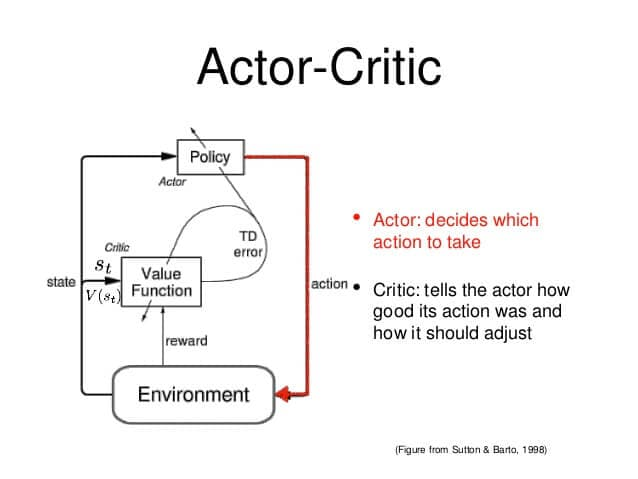
\includegraphics[width=\linewidth]{../Figures/Actor_Critic.jpg}
    \caption{The structure of Actor-Critic}
\end{figure}

As we mentioned in section 4.3.1, critic is a value-based function with parameter $w$, it could be state value function $V_w(s)$ or state-action value function $Q_w(s,a)$. Actor is a policy-based function $\pi _\theta (a|s)$ with parameter $\theta$, it updates the parameter $\theta$ according to the suggestions given by critic. The update parameter method of value-based algorithm and policy-based algorithm is mentioned in section 4.3.1.1 and 4.3.1.2.

In this paper, we used Advantage Actor-Critic(A2C). It differs from basic Actor-Critic in that the value function in critic is replaced with advantage value $A_w(s,a)$. It is defined by the following formula:
$$
A_w(s,a)=Q_w(s,a)-V_w(s)
$$

In this formula, $V_w(s)$ is the state value, which is the sum of the state-action values corresponding to all possible actions in state $s$ multiplied by the probability of taking the action, in other words, $V_w(s)=\sum_{a'\in A(s)}\pi(a'|s)\cdot Q_w(s,a')$, is a mathematical expectation. $Q_w$ is the state-action value corresponding to the action $a$ in state $s$.

So, the advantage value $A_w(s,a)$, is the advantage of current action $a$ over the average action in state $s$. If the advantage value $A_w(s,a)$ is greater than zero, then the action $a$ is better than the average action in state $s$. If the advantage function $A_w(s,a)$ is less than zero, then the current action $a$ is not as good as the average action.

However, we usually do not calculate state-action value $Q_w(s,a)$ and state value $V_w(s)$ separately. Because in this case we need to train two networks at the same time, one for calculating state-action value and one for calculating state value, which will increase the amount of calculation. 

The usual practice is to replace $Q_w(s,a)$ with $r+\gamma V_w(s')$, where $r$ is the reward obtained by the agent performing action $a$ in state $s$, $s'$ is the next state the agent moves to after performing action $a$ in state $s$ and $\gamma$ is the attenuation coefficient. In this case, we only need to train a network to calculate the state value, and the advantage value will be:
$$
A_w(s,a)=r+\gamma V_w(s')-V_w(s)
$$

Regarding the update method of policy-based algorithm, we have already mentioned it in section 4.3.1.2, in the actor it has the following form:
$$
\theta_{t+1}=\theta_t+\alpha Q_w(s,a) \nabla_\theta ln\ \pi_\theta(a_t|s_t)
$$
For the update method of value-based algorithm, critic, we only need to update according to the direction of the gradient descent of the value function:
$$
w_{t+1}=w_t+\alpha A_w(s_t,a_t) \nabla_w Q_w(s_t,a_t)
$$

%Now we should define loss function for both two networks, actor and critic. For critic, its predicted value is $V_w(s)$, the target value is $r+\gamma V_w(s')$, so we could use the mean square error of the advantage value as the loss function of critic. For actor, in discrete action space, we could think of actor as a classification task, actor should classify the action to be performed in state $s$ into the correct category. So we can calculate the actor loss like usually do for probabilities, that is using the negative log likelihood, scaled by the advantage value.

The pseudo code of A2C is shown in algorithm 4..

\begin{algorithm}
    \caption{Advantage Actor-Critic}
    \LinesNumbered
    \textbf{Initialize}{
        $\theta, w$ randomly
    } \\
    \For{$i \in [0,max\_episodes]$}{
        $s=s_0$  \\
        \While{$s$ is NOT terminal}{
            Sample action $a\ \sim\ \pi_\theta(a|s)$ \\
            Take action $a$, observe reward $r$, next state $s'$ \\
            $\theta \leftarrow \theta+\alpha Q_w(s,a) \nabla_\theta ln\ \pi_\theta(a|s)$ \\
            $A_w(s,a)=r+\gamma V_w(s')-V_w(s)$ \\
            $w \leftarrow w+\alpha A_w(s,a) \nabla_w Q_w(s,a)$ \\
            $s=s'$
        }
    }
\end{algorithm}

\subsection{Route solving}
In this section, we will introduce how to model the route problem and how to use reinforcement learning to solve it. 

Given a task graph and determined NoC architecture, when the mapping result is determined, we need to plan the route according to the transmission in the task graph. Although the start and end points have been determined, the exploration space of the route is still very large. Figure 4. shows an example. We expect to calculate a route with as little contention as possible for all transmissions.

\begin{figure}
    \centering
    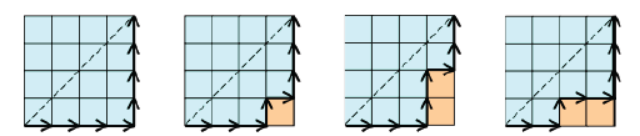
\includegraphics[width=\linewidth]{../Figures/example_for_route_space.png}
    \caption{Different route for same start and end points}
\end{figure}

Without considering going in the opposite direction of destination, the number of times of data transmission along the X or Y axis are determined. For example, the transmission in Figure 4. transmit 4 times along the X axis and 4 times along the Y axis. These two numbers are certain regardless of the route. Different routes only affect the order in which data moves along the X axis or Y axis appears during transmission. 

Based on this consideration, we only need to let our reinforcement learning model tell the data that, when it reaches a router, the next step should be along the X axis or along the Y axis. The direction of movement is towards the destination, so the data will definitely reach the destination it should go, and will not get lost in the wrong place.

Clarify the concepts in reinforcement learning, our environment is links in NoC. Some of them may have been occupied by other transmissions in a certain period of time. Given an edge $e$ in task graph that needs to calculate route, our agent is data to be transferred of this edge and the state is the use of links in NoC. Specifically, we use a $N \times 4$ matrix to represent the state. $N$ is the number of PEs, '4' represents 4 links connected to each PE (PE at the border has less than 4 links). When data arrives at a PE and starts to use a certain link connected to this PE for transmission, the corresponding position in the matrix will be set to 1. Links not used in the matrix correspond to 0.

The agent has two actions to choose from in each state, moving along the X axis or along the Y axis. This action will use the link in NoC, so after performing an action, set the corresponding position in the matrix to 1, and then move to the next state. Reward is the opposite number of contention times when transmitting in the route given by next state.

We devised a simple method to estimate contention times during transmission of a certain edge in the task graph. First, we need to record the usage status $L$ of each link,that is, during which time period the link is occupied. Given an edge $e$ that needs to calculate contention times, we find the latest available time $t_1$ among the links that need to be used by $e$ according to $L$. Then we get the completion time $t_2$ of the task corresponding to the start point of this edge. After that, we subtract $t_2$ from $t_1$ to get the estimated contention times of edge $e$.

We use breadth first search to access each edge in the task graph that needs to be calculated for the route.

Regarding the order in which we calculate the route for edges in task graph, we sort according to the end time of the start point of edges. The sooner the task is completed, the sooner the data to be sent by this task can be calculated for the route.

Figure 4. is a flowchart of the routing algorithm.

\begin{figure}
    \centering
    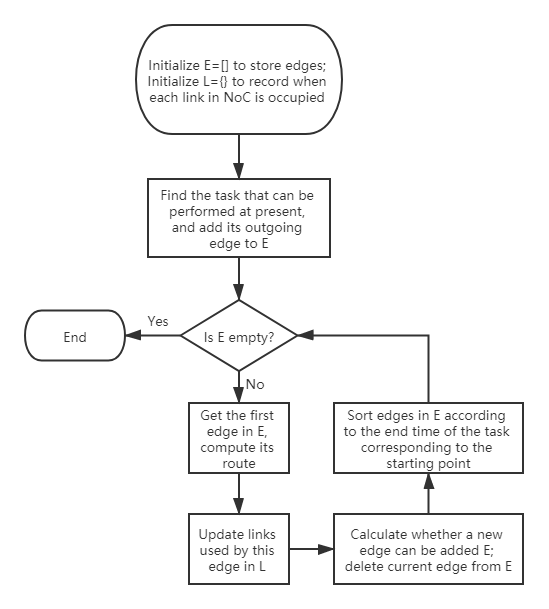
\includegraphics[width=\linewidth]{../Figures/routing.png}
    \caption{Routing algorithm}
\end{figure}